\documentclass[11pt, twoside, a4paper]{book}

\usepackage{graphicx}
\usepackage[utf8]{inputenc}
\usepackage{ngerman}
%\usepackage{lineno}
\usepackage{verbatim}
\usepackage[squaren]{SIunits}
\usepackage{amsmath}
\usepackage{amsfonts}
\usepackage{amssymb}
\usepackage{enumitem}
\usepackage{fancyhdr}
\usepackage{textcomp}
\usepackage{subcaption}
\usepackage[noadjust]{marginnote}
\usepackage{tikz}
\usepackage{nicefrac}
\usepackage{framed}
\usepackage{import}

\usetikzlibrary{calc,intersections}
\usetikzlibrary{arrows}
\usetikzlibrary{decorations.markings}
\usetikzlibrary{decorations.pathreplacing}
\usepackage[european resistors]{circuitikz}
\usepackage[ 
    top=2cm, 
    bottom=2cm, 
    outer=3cm, 
    inner=3cm,
    marginparwidth=2.5cm,
		headheight=14pt
  ]{geometry}

\usepackage{parskip}
\usepackage{pdfpages}

\setlength{\parindent}{0pt}

\newcommand{\experimentheader}[4]
{
  \iftutor{{\bf Schwierigkeitsgrad:} #1\\}
  \iftutor{{\bf Dauer:} #2\\}
  {\bf Ger\"ate:} #3\\
  {\bf Bauteile:} #4
}

\newcommand{\hintboxNone}{0}
\newcommand{\hintboxExclamation}{1}
\newenvironment{hintbox}[4][\hsize]
{
  \def\FrameCommand
  {%
    {\color{#3}\vrule width 3pt}%
    \hspace{0pt}%must no space.
    \fboxsep=\FrameSep\colorbox{#4}%
  }%
  \MakeFramed{\hsize#1\advance\hsize-\width\FrameRestore}%
  \mbox{\textbf{#2}:}%
}
{
  \endMakeFramed
}
\newcommand{\xhintbox}[3]
{
  \begin{hintbox}{Achtung}{red!50}{red!10}
    #3
  \end{hintbox}
}

\newenvironment{hint}
{
  \begin{hintbox}{Hinweis}{green!50}{green!10}
}
{
  \end{hintbox}
}

\newenvironment{definition}
{
  \begin{hintbox}{Definition\\}{white!50}{white!10}
}
{
  \end{hintbox}
}

\newenvironment{important}
{
  \begin{hintbox}{Hinweis}{gray!50}{gray!10}
}
{
  \end{hintbox}
}

\newenvironment{jason}
{
  \begin{hintbox}{Achtung}{red!50}{red!10}
}
{
  \end{hintbox}
}

\newcommand{\mandatoryenumi}
{
  \renewcommand{\labelenumi}{\arabic{enumi}.} 
}
\newcommand{\optionalenumi}
{
  \renewcommand{\labelenumi}{$\bigstar$\quad\arabic{enumi}.} 
}
\newcommand{\mandatoryenumii}
{
  \renewcommand{\labelenumii}{(\alph{enumii})} 
}
\newcommand{\optionalenumii}
{
  \renewcommand{\labelenumii}{$\bigstar$\quad(\alph{enumii})} 
}
\newcommand{\icname}[1]{\mbox{\tt #1}}


  %\newcommand{\iftutor}[1]{}
\newcommand{\ifnotutor}[1]{#1}

  \newcommand{\iftutor}[1]{#1}
\newcommand{\ifnotutor}[1]{}


\newenvironment{tutorhint}{\comment}{\endcomment}
\newenvironment{todo}{\comment}{\endcomment}
\newenvironment{solution}{\comment}{\endcomment}
\iftutor
{
  \renewenvironment{todo}
  {
    \hintbox{Todo}{red!50!yellow!90}{red!50!yellow!20}
  }
  {
    \endhintbox
  }
  \renewenvironment{tutorhint}
  {
    \hintbox{Tutorenhinweis der Stunde}{blue!50}{blue!10}
  }
  {
    \endhintbox
  }
  \renewenvironment{solution}
  {
    \hintbox{L\"osung}{black!80}{black!5}
  }
  {
    \endhintbox
  }
}
\newcommand{\etutorhint}[1]
{
  \iftutor{
    \tutorhint
      #1
    \endtutorhint
  }
}
\newcommand{\esolution}[1]
{
  \iftutor
  {
    \solution
    #1
    \endsolution
  }
}
\newcommand{\etodo}[1]
{
  \iftutor
  {
    \todo
    #1
    \endtodo
  }
}



\begin{document}

\renewcommand{\thechapter}{\arabic{chapter}}
\setcounter{chapter}{10}
\def\chaptername{Versuch}

\chapter{Thermoelement}
\label{v:11}

Ein Thermoelement wandelt Wärme in elektrische Energie um. In diesem Versuch soll das Thermoelement zur Messung einer Temperatur benutzt werden.

%------------------------------------------------
\section{Stichworte}
%------------------------------------------------

Metallbindung; Austrittsarbeit; Fermienergie; Kontaktspannung; Thermospannung; Thermoelement; W"armebad.
%
%------------------------------------------------
\section{Literatur}
%------------------------------------------------

Gehrtsen, Kapitel 6.6.1, 8.1.1, 14.1.5, 14.3.1/2\\
R. Pelster, R. Pieper, I. Hüttl, \textit{Thermospannungen - Viel genutzt und fast immer falsch erklärt!}, PhyDid 1/4 (2005)

%------------------------------------------------
\section{Anwendungsbeispiele}
%------------------------------------------------

Thermoelemente werden zur Temperaturmessung in vielen verschiedenen Umgebungen benutzt, z. Bsp. in Flüssigkeiten verschiedenster Ph-Werte, in industriellen Anwendungen mit extremen Temperaturen und Atmosphären Zusammensetzungen. Sie werden aber auch zur hochgenauen Temperaturmessung im Labor verwendet.

%------------------------------------------------
\section{Theoretischer Hintergrund}
%------------------------------------------------

\textit{Thomas Johann Seebeck} l"otete 1821 zwei Dr"ahte aus verschiedenen Metallen zu einem Ring zusammen und fand, dass eine Temperaturdifferenz zwischen den beiden L"otstellen einen Strom antreibt.\\
In vielen Lehrbüchern, auch für Experimentalphysiker, sowie in älteren Versionen dieses Skripts, wird dieses Phänomen fälschlicherweise durch die unterschiedliche Auslösearbeit der Elektronen in den beiden Metallen erklärt. In Wirklichkeit liefert diese jedoch nur einen kleinen Beitrag zum gesammten Effekt. Hier legen wir eine vereinfachte, jedoch komplette Behandlung, dar, wie sie von Pelster et al. vorgestellt wurde.

\subsection{Thermodiffusion}

Betrachten wir zunächst einen Metallstab bei konstanter Temperatur. Die freien Ladungsträger, in diesem Fall Elektronen, sind homogen im Stab verteilt und führen eine ungeordnete Wärmebewegung (s. Browne'sche Bewegung, Maxwell Verteilung). Der Betrag der mittleren Geschwindigkeit hängt dabei von der Temperatur ab: Je wärmer der Körper, desto schneller bewegen sich die Elektronen.\\
Haben die Stabenden nun unterschiedliche Temperaturen, so ist die Geschwindigkeit der Elektronen am heißen Ende höher als am kalten Ende. Dies führt zu einer gerichteten Netto-Bewegung der Elektronen vom warmen zum kalten Ende des Stabes (vgl. Diffusion). Passenderweise nennt man diese Bewegung Thermodiffusion. Sie führt dazu, dass sich das kalte Ende des Stabes gegenüber dem warmen negativ auflädt. Die Aufladung wächst solange an, bis das sich aufbauende elektrische Feld stark genug ist, die Diffusion zu kompensieren: Der Diffusionsstrom kommt zum Erliegen.\\
Die Spannung zwischen den beiden Stabenden, die sogenannte Thermodiffusionsspannung, ist in erster Näherung proportional zur Temperaturdifferenz zwischen den Stabenden:
\begin{equation}
	U_{TD} = -Q\cdot \Delta T
\end{equation}
Der Proportionalitätsfaktor $Q$, der Seebeck-Koeffizient, ist materialspezifisch, d.h. es ergeben sich unterschiedlich große Spannungen je nachdem, welches Metall (oder Halbleiter) man betrachtet.

\subsection{Thermoelement}

Fügt man zwei Teilstücke aus unterschiedlichen Materialien zu einem Ring zusammen, so ergibt sich eine Schleife mit einem thermoelektrischen Kreisstrom. Beim Thermoelement ist ein Voltmeter in die Schleife geschaltet, so dass praktisch kein Strom fließt. Das Voltmeter zeigt dann die Thermospannung, i.e. die Differenz der beiden Thermodiffusionsspannungen:
\begin{equation}
	U_{Thermo} = U^A_{TD} - U^B_{TD}.
\end{equation}
Entfernt man das Voltmeter und schliesst den Kreis, so treibt diese Thermospannung einen Kreisstrom an. Dabei bestimmt das Material mit der größeren Thermodiffusionsspannung die Stromrichtung (ähnlich wie in einem Stromkreis mit zwei ungleichen gegeneinandergeschalteten Batterien).

%Wenn zwei verschiedene Metalle 1 und 2 einander ber"uhren, gehen einige Elektronen von einem zum anderen "uber. In welche Richtung mehr Elektronen "ubergehen h"angt von den Energien der h"ochsten besetzten Energiezust"ande (Fermie-Energie), d.h. der Austrittsarbeit der Elektronen ab. Das Metall mit der geringeren Austrittsarbeit (1) gibt Elektronen ab und wird somit positiv geladen. Der "Ubertritt h"ort erst auf, wenn sich eine \textit{Kontaktspannung} aufgebaut hat, die entgegengesetzt gleich der Differenz der Austrittsarbeiten ist. Dann treten in beide Richtungen gleich viele Elektronen "uber: von 1 nach 2 durch Diffusion, von 2 nach 1 infolge des elektrischen Feldes in der Grenzschicht.\\
%In einer vereinfachenden Betrachtung beschreibt man diese beiden Elektronengase durch die Boltzmann-Statistik (in Wirklichkeit gilt f"ur so dichte Gase die Fermi-Statistik). Diese ergibt f"ur die Kontaktspannung eine Abh"angigkeit vom Verh"altnis der Teilchenzahldichten:
%\begin{equation} \label{eq:Kontaktspannung}
% \frac{n_1}{n_2} = e^{-e\,\Delta U/(kT)} \; \Rightarrow \; \Delta U = \frac{kT}{e}\ln\frac{n_2}{n_1}
%\end{equation}
%Wie man sieht, h"angt die Kontaktspannung auch von der Temperatur der Kontaktstelle ab.\\

%\noindent
%Biegt man die beide Dr"ahte zu einem Ring, so bildet sich an beiden Kontaktstellen eine Kontaktspannung aus. Da beide Spannungen aber entgegengesetzt  geschaltet sind, flie{\ss}t im Ring kein Strom.\\
%Erw"armt man aber eine der Kontaktstellen, dann werden die beiden Kontaktspannungen laut Gleichung \ref{eq:Kontaktspannung} trotz gleichen Verh"altnisses $n_2/n_1$ unterschiedlich, und es flie{\ss}t ein \textit{Thermostrom}. Die daf"ur ben"otigte Energie wird der W"armequelle entnommen.\\
%L"otet man also zwei Dr"ahte aus verschiedenen Metallen an beiden Enden zusammen und schaltet in den einen Draht ein Voltmeter, so zeigt dieses ein \textit{Thermospannung} an, die au{\ss}er von den Eigenschaften der beiden Metale nur von der Temperaturdifferenz $\Delta T$ zwischen den beiden L"otstellen abh"angt.\\
%Solche \textit{Thermoelemente}, deren eine L"otstelle auf einer konstanten Temperatur gehalten wird (z.B. durch Eintauchen in Eiswasser) sind aufgrund ihrer hohen Genauigkeit und kleinen W"armekapazit"at (und damit kleinen Tr"agheit) sehr gut als Thermometer geeignet.\\

%\noindent
%Laut Gleichung \ref{eq:Kontaktspannung} betr"agt die Thermospannung, als Differenz der beiden Kontaktspannungen:
%\begin{equation} \label{eq:Thermospannung}
% U_{th} = \frac{k}{e}\ln\frac{n_2}{n_1}\cdot \Delta T\; .
%\end{equation}
%F\"ur einige Metallkombinationen, z. B. Kupfer-Konstantan oder Eisen-Konstantan, gilt das auch in einem weiten Temperaturbereich. Die detaillierte Betrachtung mithilfe der Fermi-Statistik (die hier richtiger, aber wesentlich komplexer ist), liefert aber eine Abh"angigkeit der Thermospannung von h"oheren Potenzen von $\Delta T$, die bei sehr pr"azisen Messungen beachtet werden muss.

%------------------------------------------------
\section{Fragen zur Vorbereitung}
%------------------------------------------------

\begin{enumerate}
 %
 \item Was soll heute im Praktikum gemessen werden? Warum?
 %
 %\item Wie verhalten sich Ladungen mit gleichem bzw. ungleichem Vorzeichen?
 %
 %\item Zeichnen Sie die elektrischen Feldlinien einer Punktladung.
 %
 \item Welche Kraft wirkt auf eine elektrische Ladung in einem elektrischen Feld? Wovon h"angt die Kraft ab?
 %
 %\item Was ist ein Elektronengas?
 %
 \item Welche Bedeutung hat die Austrittsarbeit? Ist sie bei allen Metallen gleich?
 %
 %\item Wie ist die Fermi-Energie definiert?
 %
 \item Warum tritt eine Kontaktspannung auf, wenn sich zwei unterschiedliche Metalle ber"uhren?
 %
 \item Wie ist ein Thermoelement aufgebaut? Wie erzeugt es die Thermospannung?
 %
\end{enumerate}

%------------------------------------------------
\section{Durchführung} 
%------------------------------------------------

\begin{hint}
Bitte achten Sie darauf, dass keine der Kabel mit der heißen Kochplatte in Berührung kommen!
\end{hint}

\begin{enumerate}
 %
 \item Tauchen Sie die Lötstellen des Thermoelements in Eiswasser. Messen Sie die Thermospannung.
 %
 \item Erhitzen Sie nun das Wasserbad langsam bis das Wasser siedet. Messen Sie während des Erhitzens die Thermospannung f"ur Temperaturen in Schritten von $5^{\circ}$\,C.
 
 \noindent
 \textbf{Beachten Sie:} Die Herdplatte wird kurz auf Stufe 12 betrieben. Der komplette Versuch ist schon fertig aufgebaut, es muss nichts mehr angeschlossen werden!\\
 Stellen Sie das Thermometer nicht auf den Gef"a{\ss}boden! Die Kabel d"urfen die Herdplatte nicht ber"uhren.\\
 Eine langsamere Erw"armung des Wassers erlaubt eine genauere Messung.
 %
 \item Setzen Sie die Messung fort, während das Wasser wieder abkühlt. \\
 Der Abkühlungsprozess kann durch Zugabe von Eisstücken beschleunigt werden.
 
 \noindent
 \textbf{Beachten Sie:} Das Wasser muss zur gleichmäßigen Temperaturänderung mit einem Glasstab in Bewegung gehalten werden.
\end{enumerate}
\begin{figure}[h!]
	\centering
		%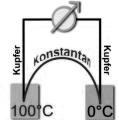
\includegraphics[width=0.15\textwidth]{Versuch_11-12/Abbildungen/Messung.JPG}
		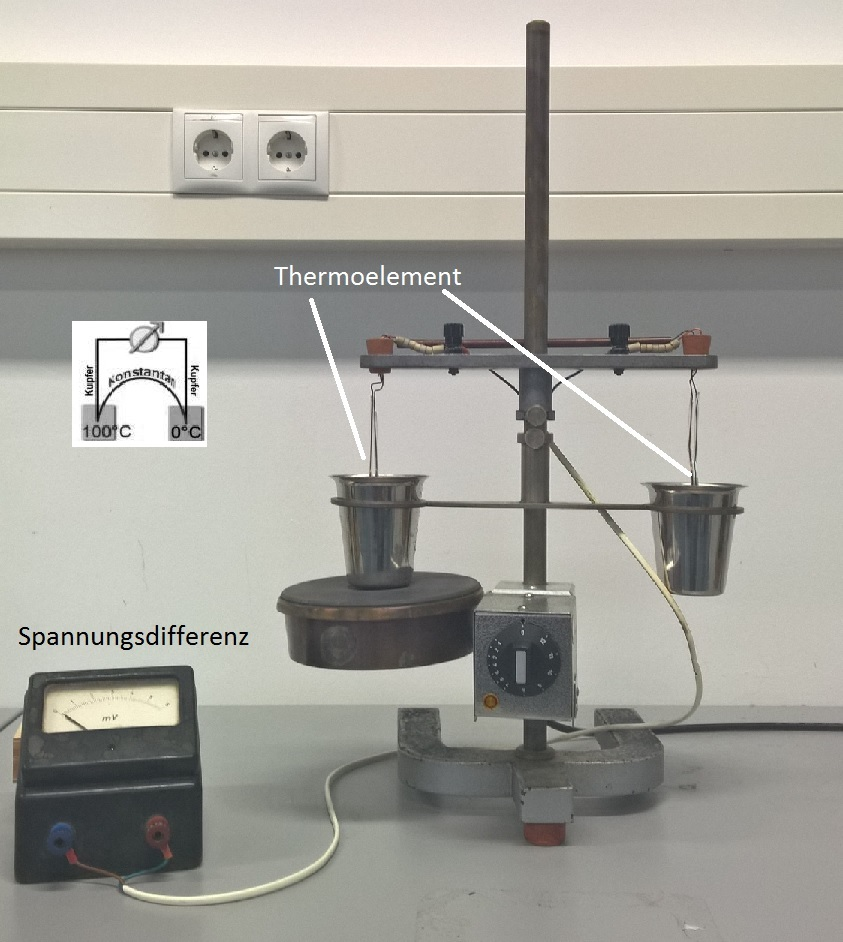
\includegraphics[width=0.75\textwidth]{Abbildungen/Thermoelement_Aufbau2.JPG}
	\caption{Messaufbau}
	\label{fig:Messung}
\end{figure}
%------------------------------------------------
\section{Auswertung} 
%------------------------------------------------
\etodo{Musterauswertung}

\begin{hint}
	Bitte fertigen Sie die Graphen in der folgenden Auswertung per Hand auf Millimeterpapier an.
\end{hint}

\begin{enumerate}
 %
 \item Stellen Sie die Thermospannung in mV als Funktion der Temperatur $T$ grafisch dar. Tragen Sie die Kurven f"ur Aufw"armung und Abk"uhlung des Wasserbades getrennt auf. \label{Aufg:a}
 %
 \item Lesen Sie aus der Auftragung die Empfindlichkeit des Thermoelementes ab. Sch"atzen Sie ihren Fehler aus den Grenzgeraden ab.\\
 Alle Geraden, auch die Grenzgeraden, m"ussen dabei durch den Ursprung gehen. Wieso?
 %
 \item Berechnen Sie den gewichteten Mittelwert der Empfindlichkeit des Thermoelementes. Die Formeln finden Sie im Skript.
 %
 \item Warum liegen die Geraden aus Aufgabe \ref{Aufg:a} nicht aufeinander?
 %
 \item Diskutieren Sie die Fehlerquellen in Ihrer Messung.
\end{enumerate}

\end{document}